\documentclass[11pt,a4paper]{article}
\usepackage[left=2.5cm,top=2cm,right=2.5cm,nofoot]{geometry}
\usepackage{geometry}
\usepackage{amsmath}
\usepackage{amssymb}
\usepackage{txfonts}
\usepackage{microtype}
\usepackage{epsfig}
\usepackage{graphicx}
\usepackage{moreverb}
\usepackage{hyperref}
\usepackage{listings}
\usepackage{xcolor}
\usepackage{textcomp}
\usepackage{makecell}
\usepackage{wasysym}
\definecolor{listinggray}{gray}{0.98}
\definecolor{lbcolor}{rgb}{0.98,0.98,0.98}
\lstset{
	backgroundcolor=\color{lbcolor},
	tabsize=4,
	rulecolor=,
	language=matlab,
    basicstyle=\scriptsize\ttfamily,
    upquote=true,
    aboveskip={1.5\baselineskip},
    columns=fixed,
    showstringspaces=false,
    extendedchars=true,
    breaklines=true,
    prebreak = \raisebox{0ex}[0ex][0ex]{\ensuremath{\hookleftarrow}},
    frame=single,
    showtabs=false,
    showspaces=false,
    showstringspaces=false,
    identifierstyle=\ttfamily,
    keywordstyle=\color[rgb]{0,0,1},
    commentstyle=\color[rgb]{0.133,0.545,0.133},
    stringstyle=\color[rgb]{0.627,0.126,0.941},
}

\usepackage{eso-pic}
\usepackage{ifthen}

\usepackage[nottoc]{tocbibind}
\usepackage[backend=biber,style=numeric,sorting=none]{biblatex}
\addbibresource{bibben.bib}

\usepackage{float}
\usepackage{subcaption}
\usepackage{gensymb}
\usepackage{siunitx}
\usepackage{enumitem}

\newlength\fwidth

\title{Project 1: Cosmological models}
\author{Kevin Andersson - CID: kevinan -- Eric Lindgren - CID: ericlin}
\date{November 2020}

\begin{document}

\maketitle
\pagenumbering{gobble}% Remove page numbers (and reset to 1)
\clearpage

\pagenumbering{arabic}% Arabic page numbers (and reset to 1)
\setcounter{page}{1}
\section{Introduction and Background}
In modern cosmology, scientist believe that the universe is expanding and that this expansion rate may not be constant. To describe this phenomenon scientist uses the Einstein equation of general relativity and the Robertson-Walker metric to derive the Friedman equation 
\begin{equation}
    \label{eq:friedman}
    1 = \Omega_{M} + \Omega_{k} + \Omega_{\Lambda}.
\end{equation}
$\Omega_M$ is dimensionless matter density parameter, $\Omega_\Lambda$ is related to the dark energy density and $\Omega_k$ to the topology of the universe i.e negative, positive or zero curvature. One way of examine the expansion of the universe is to look at supernovas far away, which all explode with the same luminosity. One can therefore study the distance and red shift of the supernova and relate this to the the Hubble parameter via the Friedman equations. Some alterations in the Friedman equation due to for example including radiation densities and dark-energy equation of state leads to different cosmological models. Two of them are reduced $\Lambda$CDM and $w$CDM, both of which assumes a flat space time. The two cosmological models differ in the way they relate the Hubbel parameter to the red shift $H(z) = H_0\sqrt{E(z)}$, which is described by equations \eqref{eq:lambda_model} and \eqref{eq:omega_model} \cite{project_pm}.

%We are to compare two cosmological models, $\Lambda$CDM and $w$CDM, which give different expressions for $E(z)$. These are given in equations \eqref{eq:lambda_model} and \eqref{eq:omega_model} \cite{project_pm}. $\Lambda$CDM describes a flat cosmology, whilst $w$CDM includes a dark energy equation of state. Note that $\Lambda$CDM is a two-parameter model and that $w$CDM is a three-parameter model, and that $w$CDM reduces to $\Lambda$CDM for $w=-1$. 

\begin{align}
    \label{eq:lambda_model}
    \Lambda\text{CDM}: \hspace{10px} E(z) &= \Omega_{M,0}(1+z)^3 + \Omega_{\Lambda,0} \\
    \label{eq:omega_model}
    w\text{CDM}: \hspace{10px} E(z) &= \Omega_{M,0}(1+z)^3 + \Omega_{\Lambda,0}(1+z)^{3(1+w)} 
\end{align}
%Furthermore, the parameters $\Omega_{M,0}$ and $\Omega_{\Lambda,0}$ should sum to one according to the Friedman equation $1 = \Omega_{M,0} + \Omega_{\Lambda,0} + \Omega_{k,0}$ in our case, since $\Omega_{k,0} = 0$ \cite{project_pm}.
Our goal is to use the SCP 2.1 data set over red shift and distance modules from different supernovas and perform a Bayesian analysis to examine the properties of the universe, primarily to do inference on the Hubble constant $H_0$ and the decelerating parameter $q_0$. We then also want to compare the two cosmological models $\Lambda$CDM and $w$CDM in relation to the data.


\section{Methodology}
In this short section we present our general approaches for the two tasks at hand.

\subsection[Task 1]{Task 1: Inference in the low-$z$ regime}
We are tasked with performing Bayesian anlysis to extract the joint probability distribution for $H_0$ and $q_0$. For this we have the model for the distance modules
\begin{equation*}
    \mu(z) = 5\log_{10}(d_L(z)) + 25.
\end{equation*}
Where the distances $d_L$ between earth and the can be supernova calculated as
\begin{equation}
    \label{eq:dl}
    d_L(z) = (1 + z )\int_0^z \frac{dz'}{H(z')},
\end{equation}
where $H$ is the Hubble parameter and $z$ is the red shift. For small $z$ we can perform a Taylor expansion and get the distances as 
\begin{equation*}
    d_L(z) \approx \frac{c}{H_0} \left(z + \frac{1}{2}(1 - q_0)z^2 \right),
\end{equation*}
where the decelerating parameter $q_0 = \frac{1}{2}(\Omega_M - 2 \Omega_\Lambda)$. We then want to use Bayesian analysis to fit this model $M(H_0,q_0; z) = \mu(z)$ to observed data. Lets define a parameter vector $\theta = (H_0, q_0)$; we then have the relation between our model and measured data as
\begin{equation*}
    \mu_i = M(\theta; z_i) + \varepsilon_i + \delta(z_i),
\end{equation*}
where $d_i$ is measured data of $\mu$, $\varepsilon_i$ the measurement uncertainty associated with $d_i$ and $\delta(z_i)$ is the model discrepancy. If we assume that the overall theory is accurate we can drop the model discrepancies since the Taylor expansion should be valid for small $z$. We then assume heteroscedastic, independent and identically distributed errors, i.e $\varepsilon_i \sim N(0, \sigma_i)$. From this assumption we can later write down our likelihood. But we first turn to determine the standard deviations $\sigma_i$. Our data, that are taken from measurement, comes with some error bars, $\delta_d$, which is the "sum" of all uncertainty in the experiments. This measured uncertainty for each datum gives us, for each measured datum, relative to all other data points, an uncertainty between the data and our model. To incorporate that there might be an overall scaling of these uncertainties we take $\sigma_i^2 = \sigma^2 \delta_{d_i}^2 \frac{1}{n_d}\sum \frac{1}{\delta_d^2} = \sigma W^{-1}$ and treat $\sigma$ as an unknown parameter in our Bayesian analysis. Here $W$ is the weight vector and we have normalized it to sum to $n_d$, i.e. the number of data points used.
%Note also that the data was given to us via the distance modules and its uncertanties, so we calculated $d_L$ and its uncertenty via
%\begin{equation*}
%\begin{split}
%    d_L &= 10^{\frac{\mu}{5} - 5}\\
%    \delta(d_L) &= \frac{\partial d_L}{\partial \mu} \delta(\mu).
%\end{split}
%\end{equation*}
\\\\
So to get the joint probability distribution of our parameter we use Bayes theorem 
\begin{equation*}
    P(\theta| D, I) =  \frac{p(D|\theta, I)p(\theta|I)}{p(D)}.
\end{equation*}
We get, through the iid assumption, our likelihood as
\begin{equation*}
    p(D|\theta) =  \prod_i p(d_i|\theta) = \text{exp}\left(-\sum_i \frac{1}{2\sigma_i^2}\left[d_i - M(\theta;z_i)\right]^2\frac{}{}\right) =  \text{exp}\left(-\sum_i \frac{W}{2\sigma^2}\left[d_i - M(\theta;z_i)\right]^2\frac{}{}\right).
\end{equation*}
For $H_0$ we used a uniform prior between 50 and 100 km/s/Mpc and for $q_0$ we used an uniform prior between -2 and 2. The chosen prior for $H_0$ is motivated from that all large controversies regarding the value of $H_0$ during the 2000-century has put it somewhere in between 50 and 100 km/s/Mpc \cite{}. The prior for $q_0$ comes from the assumption that the Friedman equation puts $\Omega_M$ and $\Omega_\Lambda$ in the order of 1 and that they can't be negative \cite{}. For the unknown error scale we used a inverse gamma prior with parameters $\alpha = 0.12185$ and $\beta = 2.46569$. Since we for now only are interested in relative probabilities we neglect the overall normalisation, i.e the marginal likelihood. We thus have an expression of our full posterior which we now need to sample. To sample the posterior we used the NUTS sampling algorithm, which is the No-U-Turn algorithm in Hamiltonian Monte Carlo. Using this algorithm we started four walkers which took 1000 burn-in steps and 4000 sampling steps each, and using the traces of the walkers we could extract our joint posterior distribution. We where also tasked with checking if we found convincing evidence that the acceleration of the expansion of the universe. The acceleration of the expansion is described by $q_0$ and the expansion is accelerating if it is smaller then zero and decelerating if it is larger. To draw this conclusion we needed to know the probability distribution over $q_0$ which we got from marginalising our posterior over the other parameters
\begin{equation*}
    p(q_0|D,I) = \int p(q_0,H_0, \sigma|D,I) d H_0 d\sigma.
\end{equation*}
\newline
\\\\
After this we also want to do a posterior predictive plot over the distance modules against the red shift. A posterior predictive distribution over the distances is extracted by evaluating the integral 
\begin{equation*}
    p(\mu| D) = \int p(\mu|\theta, \sigma, D) p(\theta, \sigma| D) d\theta d\sigma,
\end{equation*}
where $ p(\theta, \sigma| D)$ is the posterior and $p(\mu|\theta, \sigma, D)$ is the likelihood. To plot the posterior predictive we want to sample the posterior predictive distribution which we do by drawing many samples of $\theta$ and $\sigma$ from our posterior.  We then evaluating $\mu$ for all these samples as 
\begin{equation*}
    \mu(z) = M(\theta, z) + \varepsilon, \quad \varepsilon \sim N(0, \sigma),
\end{equation*}
and the histogram of $\mu$ for every $z$ represent our predictive distribution. 


%\begin{equation*}
%    d_L = \varepsilon  + \int d_L(\theta) p(\theta| D) d\theta.
%\end{equation*}

\subsection[Task 2]{Task 2: Model comparison of $\Lambda$CDM and $w$CDM}

The second part to analyse is to compare the two cosmological models $\Lambda$CDM and $w$CDM, defined in equations \eqref{eq:lambda_model} and \eqref{eq:omega_model}. Note that according to the Friedman equation and under the assumption of a flat universe, $\Omega_{\Lambda,0}=1-\Omega_{M,0}$. Furthermore, we interpreted the parameter $w$ in the $w$CDM-model as a model parameter, not as a hyperparameter, and it was thus inferred in the same manner as $\Omega_{M_0}$. This means that $\Lambda$CDM is a single-parameter model and $w$CDM is a two-parameter model in our implementation.

We utilised all the given data over the whole $z$-regime for the model comparison, and thus we had to numerically calculate the integral in equation \eqref{eq:dl}. As in the previous task, we start by defining the priors, likelihoods and posteriors for the two models, which are given in equations \eqref{eq:prior_lambda}-\eqref{eq:post_omega}. Note that $\theta_\Lambda=\Omega_{M,0}$, $\mu_{\Lambda}$ and $\theta_w=(\Omega_{M,0}, w)$, $\mu_{w}$ are the parameter vectors and expressions for the distance modulus $\mu(z)$ respectively, for each of the two models $M_{\Lambda CDM}$ and $M_{wCDM}$. Furthermore, we used the log of these distributions in the code implementation to improve numerical stability. 

\begin{align}
    \label{eq:prior_lambda}
    &\hspace{10px}                            \text{Priors}:  &\Omega_{M_0} \sim \mathcal{U}(0,1) \\
    \label{eq:like_lambda}
    \Lambda\text{CDM}&\hspace{10px}           \text{Likelihood}:  &p\left(\mathcal{D} \left. \right\vert \mu_{\Lambda}, \theta_{\Lambda}, I \right)  = \mathcal{N}\left( \left.\mathcal{D} \right\vert \mu_{\Lambda}(z, \theta_{\Lambda}), \Sigma\right)\\
    \label{eq:post_lambda}
    &\hspace{10px}                            \text{Posterior}: &p\left(\theta_{\Lambda} \left. \right\vert \mathcal{D}, M_{\Lambda CDM}, I \right) \propto p\left(\mathcal{D} \left. \right\vert \mu_{\Lambda}, \theta_{\Lambda}, I \right) p\left(\theta_{\Lambda} \right)\\
    \label{eq:prior_omega}
    &\hspace{10px}                            \text{Priors}:  &\Omega_{M_0} \sim \mathcal{U}(0,1), \hspace{5px} w \sim \mathcal{U}(-10,10) \\
    \label{eq:like_omega}
    w\text{CDM}& \hspace{10px}                \text{Likelihood}:  &p\left(\mathcal{D} \left. \right\vert \mu_{w}, \theta_{w}, I \right)  = \mathcal{N}\left( \left.\mathcal{D} \right\vert \mu_{w}(z, \theta_{w}), \Sigma\right)\\
    \label{eq:post_omega}
    &\hspace{10px}                            \text{Posterior}: &p\left(\theta_{w} \left. \right\vert \mathcal{D}, M_{wCDM}, I \right) \propto p\left(\mathcal{D} \left. \right\vert \mu_{w}, \theta_{w}, I \right) p\left(\theta_{w} \right)
\end{align}
Note that we assume heteroscedastic errors, but with a known error scale as compared to an unknown one in the previous task. Thus, the covariance matrix $\Sigma$ only has the measurement errors $\sigma_i^2$ on the diagonal. This knowledge of the measurement errors is expressed by conditioning the distributions in equations \eqref{eq:prior_lambda}-\eqref{eq:post_omega} on $I$. $\Omega_{M_0}$ was given a $\mathcal{U}(0,1)$ prior, since it corresponds to the dimensionless matter density parameter which means that they are non-negative, and according to the Friedman equation it cannot exceed 1, since that would imply a negative dark energy density $\Omega_{\Lambda,0}=1-\Omega_{M,0}$. $w$ was described using a $\mathcal{U}(-10,10)$ prior since we expected $w$ to be in the vicinity of $w=-1$ at which $w$CDM reduced to $\Lambda$CDM and we thus assume $w$ to not differ too far from this value, since $\Lambda$CDM and $w$CDM are expected to describe the same data.


We now turn to the comparison of the $\Lambda$CDM- and $w$CDM models. A straightforward method for comparing two models $M_1$ and $M_2$ is to compute their respective marginal likelihoods for some collected data $\mathcal{D}$, $p\left(\mathcal{D} \vert M, I \right)$ \cite{lec3}. However, this requires marginalizing over the model parameters $\theta$, which may be intractable in practice. An alternative method for model comparison is the use of Information Criteria (IC), which are methods for scoring and ranking models \cite{lec3}. We specifically used the Akaike Information Criterion (AIC) and the Bayesian Information Criterion (BIC), which both are approximations valid in the large data limit. AIC and BIC are given in equations \eqref{eq:AIC} and \eqref{eq:BIC}. 

\begin{align}
    \label{eq:AIC}
    \text{AIC} &= 2 \log{p\left(\mathcal{D} \vert \theta_{\star} \right)} - 2n_p \\
    \label{eq:BIC}
    \text{BIC} &= 2 \log{p\left(\mathcal{D} \vert \theta_{\star} \right)} - 2n_p \log{n_d},
\end{align}
where $p\left(\mathcal{D} \vert \theta_{\star} \right)$ is the likelihood for data $\mathcal{D}$ evaluated at the maximum likelihood estimator (MLE) $\theta_\star$, i.e. the maximum likelihood value. $n_p$ is the number of model parameters, and $n_d$ is the number of data points. Note that both the AIC and BIC scores are defined such that a higher score indicates a better model \cite{lec3}. As a first step of the model comparison process, the AIC and BIC scores for the two models as given in equations \eqref{eq:AIC} and \eqref{eq:BIC} were computed. The maximum likelihood value enters in both AIC and BIC, which we retrieved by minimizing the negative logarithm of the likelihoods defined in equations \eqref{eq:like_lambda} and \eqref{eq:like_omega}, using the \texttt{minimize} optimizer from SciPy \cite{scipy_min}. The starting point values for the minimization was $\Omega_{M_0}=0.5$ and $w=-1$, since these points corresponds to roughly the middle of their respective priors. 

To further the model comparison we also studied the central values for the matter density parameter $\Omega_M$ and the dark energy parameter $\Omega_\Lambda$. To this end we sampled the posterior using MCMC (implemented in \texttt{emcee} in Python) for both models, and calculated the respective mean and the median values of $\Omega_{M,0}$ over these samples, from which we could calculate the values for $\Omega_{\Lambda,0}$. The mode values where obtained as the MLE from maximizing the likelihoods in obtaining the AIC and BIC scores, since in our case of uniform priors the MLE will be equal to the MAP estimates. The MCMC sampler was run with 1000 burn-in steps (i.e. steps that were discarded) and 20000 sampling steps. 

Lastly, the posterior samples from the $\Lambda$CDM-model where used to obtain the marginal posterior distribution for $\Omega_{M_0}$, $p\left(\Omega_{M_0}\vert \mathcal{D} M_{\Lambda CDM} I\right)$. This was extracted from the MCMC samples by creating a histogram from the chain of obtained $\Omega_{M_0}$ values.

\section{Results and discussion}

\subsection[Task 1]{Task 1: Inference in the low-$z$ regime}
In figure \ref{fig:Joint_dist} the joint distribution of $H_0$, $q_0$ and $\sigma$ is represented as a corner plot. We can see from the plot that  the marginalized distribution resembles a normal distribution which indicates our sampling is converged, at least if there does not exist other modes in the distribution. We can also see that $\sigma^2$ seems to be independent of $H_0$ and $q_0$ while $H_0$ and $q_0$ seems to be correlated. This is however very reasonable since in our model we have a term with $\frac{q_0}{H_0}$ so if $H_0$ increases then the magnitude of $q_0$ also does which we observe in the figure. We can also see from the distribution marginalized  over $H_0$ and $\sigma$ that all probability density of $q_0$ lies below zero, with a mode at $-0.42$ and a standard deviation of $\pm 0.09$. We can thus with very high belief draw the conclusion that the universes expansion is accelerating.  
% \begin{figure}[H]
%     \centering
%     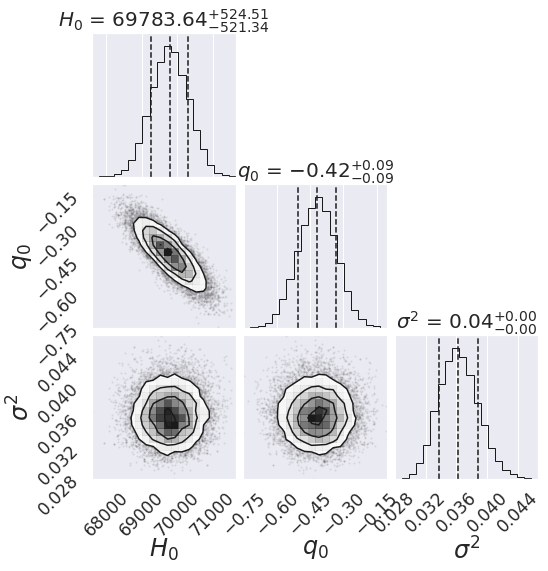
\includegraphics[width = 0.8\textwidth]{figures/corner.png}
%     \caption{Caption}
%     \label{fig:Joint_dist}
% \end{figure}
% \ref{fi}

\begin{figure}[H]
    \centering
    \begin{subfigure}{.55\textwidth}
          \centering
          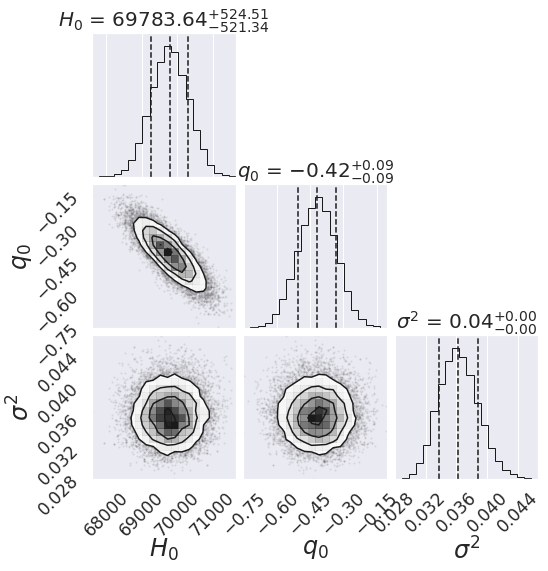
\includegraphics[width=0.9\linewidth]{figures/corner.png}
          \caption{Caption}
          \label{fig:Joint_dist}
    \end{subfigure}%
    \begin{subfigure}{.45\textwidth}
          \centering
          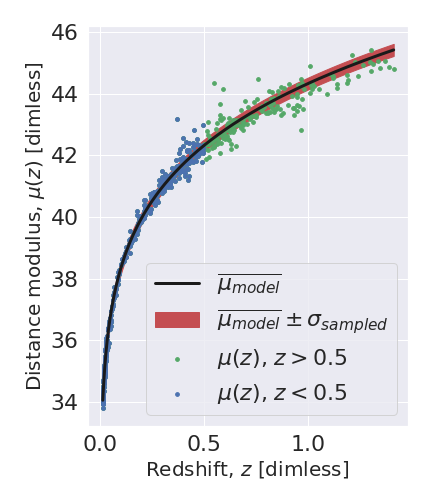
\includegraphics[width=0.9\linewidth]{figures/predictive_plot_mu.png}
          \caption{Caption}
          \label{fig:posterior_pred}
    \end{subfigure}
    \caption{Caption.}
    \label{fig:posterior_task1}
\end{figure}

In figure \ref{fig:posterior_pred} we can see our posterior predictive plot with the mean prediction and with the standard deviation uncertainty. We see that our prediction coincide very well with our data in the low regime and the errors there are also relatively small. For higher $z$ our prediction may be slightly off and we see that our uncertainty gets slightly bigger. This is reasonable since we have not fitted to data in this regime and our model also breaks down since we assumed low $z$ in the Taylor expansion. We also see that for very low $z$ the fit seems very accurate, since we here also can neglect the second order term in $z$ this indicate that $H_0$ has a reasonable fit. An interesting thing to note is that the broader uncertainty for larger $z$ in the posterior predictive only arise from our uncertainty of our parameters $\theta$. The data uncertainty $\sigma$ is in this framework constant for all $z$ in spite the fact that data errors seem to get slightly larger for larger $z$. We are not convinced that this is is a problem or not and some feedback regarding this would be appreciated.
% \begin{figure}[H]
%     \centering
%     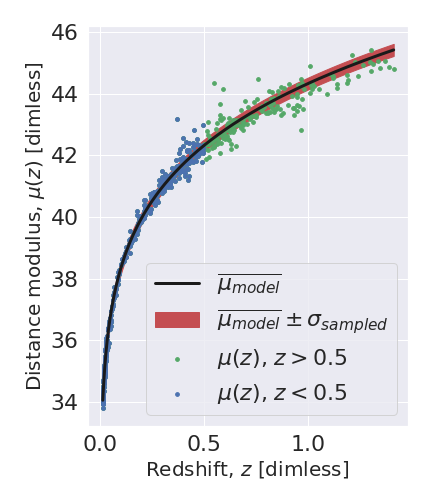
\includegraphics[width = 0.8\textwidth]{figures/predictive_plot_mu.png}
%     \caption{Caption}
%     \label{fig:posterior_pred}
% \end{figure}
There are a number of ways of how to improve the inference of $H_0$ and $q_0$. The first thing one should think about is the choice of priors. We have chosen relatively broad uniform priors, but one might perhaps already from the theory conclude lower bounds for the parameters. One could also consider Gaussian or other types of priors where we could have more probability density close to the parameter value we believe to be true. In these cases one could also use hyperpriors to incorporate uncertainty in the parameters of our priors. The very best way to define the prior could also be to use the posterior of some previous analyses where one perhaps used different data or estimated the parameters in a different way. The next thing one should think about is what kind of model discrepancies one has. In this case we have introduced discrepancies when performing the Taylor expansion, possibly also when assuming a flat universe and probably many more of varying importance (Einstein gravity only low energy approximation of string theory). One might then consider to extend the model to incorporate more terms in the expansion, do the full integral or include open and flat universes. If this not is possible one could also try to model the discrepancy with a Gaussian process where one might be able to use some information one have about the discrepancy to advantage, for example $\delta(z = 0) = 0$. And lastly the inference would also be better if one include more data, and can reduce the uncertainty in the data. Additional data to the inference could also be of other kinds like mention in the PM the angular power spectrum of the cosmic microwave background could also be used to test cosmological models. 



\subsection[Task 2]{Task 2: Model comparison of $\Lambda$CDM and $w$CDM}

\begin{table}[H]
    \centering
    \caption{Obtained AIC and BIC scores for the different models, as well as the maximum likelihood estimates (MLE) for the model parameters in each case.}
    \begin{tabular}{||c | c c | c c c||} 
         \hline
         Model & AIC & BIC & $\Omega_{M,0, MLE}$ & $\Omega_{\Lambda, 0, MLE}$ & $w_{MLE}$\\ [0.5ex] 
         \hline\hline
         $\Lambda$CDM & 235.48 & 231.12 &   0.278 & 0.722 &  \\
         \hline
         $w$CDM & 233.48 & 224.76 & 0.280 &  0.720 & -1.0004 \\ [0.5ex]
         \hline
    \end{tabular}
    \label{tab:AIC_BIC}
\end{table}


The obtained AIC and BIC scores together with the maximum likelihood estimates (MLE) of the parameters as obtained from maximizing the (log) likelihood using Scipy are given in table \ref{tab:AIC_BIC} above. As before, the dark energy density is estimted as $\Omega_{\Lambda,0, MLE}=1-\Omega_{M,0, MLE}$. We observe that $\Lambda$CDM achieves a higher score than $w$CDM, indicating that $\Lambda$CDM is a better model for describing the data. This may largely be due to the extra parameter in $w$CDM; the extra degree of freedom that $w$CDM has in explaining the data due to the parameter $w$ does not seem to yield a significant enough benefit to compensate for the cost of adding this extra parameter. Because of this, we would expect $w$CDM to overfit to the data to a higher degree than $\Lambda$CDM. 

\begin{table}[H]
    \centering
    \caption{Obtained posterior central values for $\Omega_{M,0}$ and $\Omega_{\Lambda,0}$ for the two models. Note that all central values are similar in magnitude, which indicates a unimodal distribution for $\Omega_{M,0}$.}
    \begin{tabular}{||c | c c | c c | c c||} 
         \hline
         Model & Mean $\Omega_{M,0}$ & Mean $\Omega_{\Lambda,0}$ & Mode $\Omega_{M,0}$ & Mode $\Omega_{\Lambda,0}$ & Median $\Omega_{M,0}$ & Median $\Omega_{\Lambda,0}$ \\ [0.5ex] 
         \hline\hline
         $\Lambda$CDM & 0.2781 & 0.7219 & 0.2778 & 0.7223 & 0.2779 & 0.7221 \\
         \hline
         $w$CDM & 0.2781 & 0.7219 & 0.2796 & 0.7204 & 0.2839 & 0.7161 \\ [0.5ex] 
         \hline 
    \end{tabular}
    \label{tab:central_values}
\end{table}

Moving on to the model parameter inference and analysis, the obtained posterior central values for $\Omega_{M,0}$ and $\Omega_{\Lambda,0}=1-\Omega_{M,0}$ are given in table \ref{tab:central_values}. The central values are all very similar, which indicates that the posterior distribution for $\Omega_{M,0}$ is unimodal and fairly symmetric regardless of the model used, which indicates that both models describe the data in a similar fashion. These central values are somewhat in line with estimates for $\Omega_{M,0}$ from more extensive analysis; the Planck 2018 collaboration obtained $\Omega_{M,0} = 0.321 \pm 0.013$ and $\Omega_{\Lambda,0} = 0.679 \pm 0.013$ \cite{planck} (68\% limits), a compilation of measurements from LAMBDA NASA reports values in the range $\Omega_{M,0}\in \left[0.27, 0.33 \right]$ \cite{lambdanasa} and COSMOS which reports $\Omega_{\Lambda,0} = 0.73$ \cite{cosmos}.

Studying the posterior distribution for $\Omega_{M,0}$ in figure \ref{fig:posterior_task2}, we observe that the distribution is indeed unimodal and centered around $\Omega_{M,0}\approx0.28$. A 90\% highest posterior density (HPD) region is given by $\Omega_{M,0} \in [0.257, 0.300]$. Note that this includes some of the results from more extensive analysis, but not all of them.

Our results, regarding the inference for $\Omega_{M,0}$ and $\Omega_{\Lambda,0}$, as well as comparison with other sources, indicates that we indeed live in a dark energy dominated universe, with only about $\approx 28\%$ of the universe being made up of matter.

\begin{figure}[H]
    \centering
    \begin{subfigure}{.5\textwidth}
          \centering
          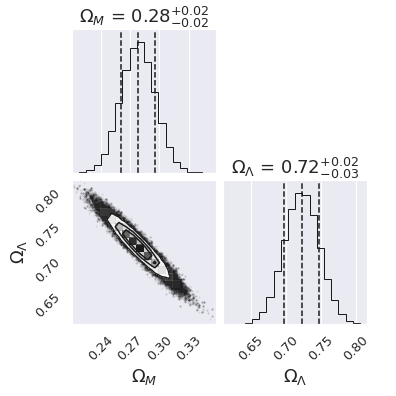
\includegraphics[width=0.9\linewidth]{figures/corner_task2.png}
          \caption{Corner plot of $p\left(\Omega_{M,0},\Omega_{\Lambda,0} \left. \right\vert D, M_{\Lambda CDM} I \right)$}
          \label{fig:sub1}
    \end{subfigure}%
    \begin{subfigure}{.5\textwidth}
          \centering
          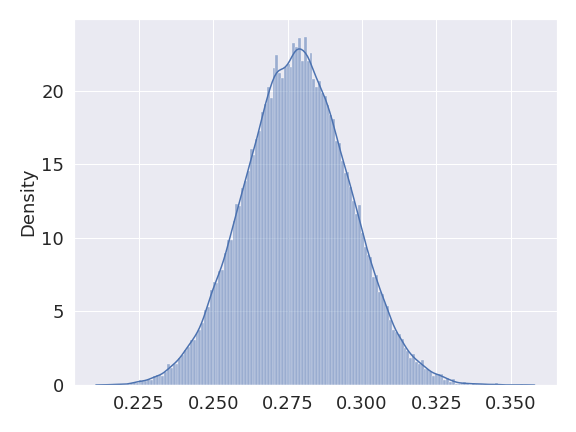
\includegraphics[width=0.9\linewidth]{figures/posterior_task2.png}
          \caption{$p\left(\Omega_{M,0} \left. \right\vert D, M_{\Lambda CDM} I\right)$}
          \label{fig:sub2}
    \end{subfigure}
    \caption{Posterior distribution for for $\Omega_{M,0}$ with a 90\% highest posterior density (HPD) interval. Note that the distribution is unimodal and symmetric.}
    \label{fig:posterior_task2}
\end{figure}

\printbibliography

\end{document}
